\section{Introduction}
% Chris: 1) emphasize why it is an important problem 2) why RC isn't solved and motivated the need for big training data, which motivate looking at Deepmind Data. 3) raise questions about that dataset and the approaches so far 4) outline our models and results

Reading comprehension (RC) is the ability to read text, process it, and understand its meaning.\footnote{\url{https://en.wikipedia.org/wiki/Reading_comprehension}} How to endow computers with this capacity has been an elusive challenge and a long-standing goal of Artificial Intelligence (e.g., \cite{norvig87phd}). Genuine reading comprehension involves interpretation of the text and making complex inferences. Human reading comprehension is often tested by asking questions that require interpretive understanding of a passage, and the same approach has been suggested for testing computers \cite{burges2013towards}.

In recent years, there have been several strands of work which attempt to collect human-labeled data for this task -- in the form of document, question and answer triples --  and to learn machine learning models directly from it \cite{richardson2013mctest,berant2014modeling,wang2015machine}. However, these datasets consist of only hundreds of documents, as the labeled examples usually require considerable expertise and neat design, making the annotation process quite expensive.  The subsequent scarcity of labeled examples prevents us from training powerful statistical models, such as deep learning models, and would seem to prevent a system from learning complex textual reasoning capacities.

Recently, researchers at \ti{DeepMind} \cite{hermann2015teaching} had the appealing, original idea of exploiting the fact that the abundant news articles of \ti{CNN} and \ti{Daily Mail} are accompanied by bullet point summaries in order to heuristically create large-scale supervised training data for the reading comprehension task. Figure~\ref{fig:example} gives an example. Their idea is that a bullet point usually summarizes one or several aspects of the article. If the computer understands the content of the article, it should be able to infer the missing entity in the bullet point.

\begin{figure}
\centering
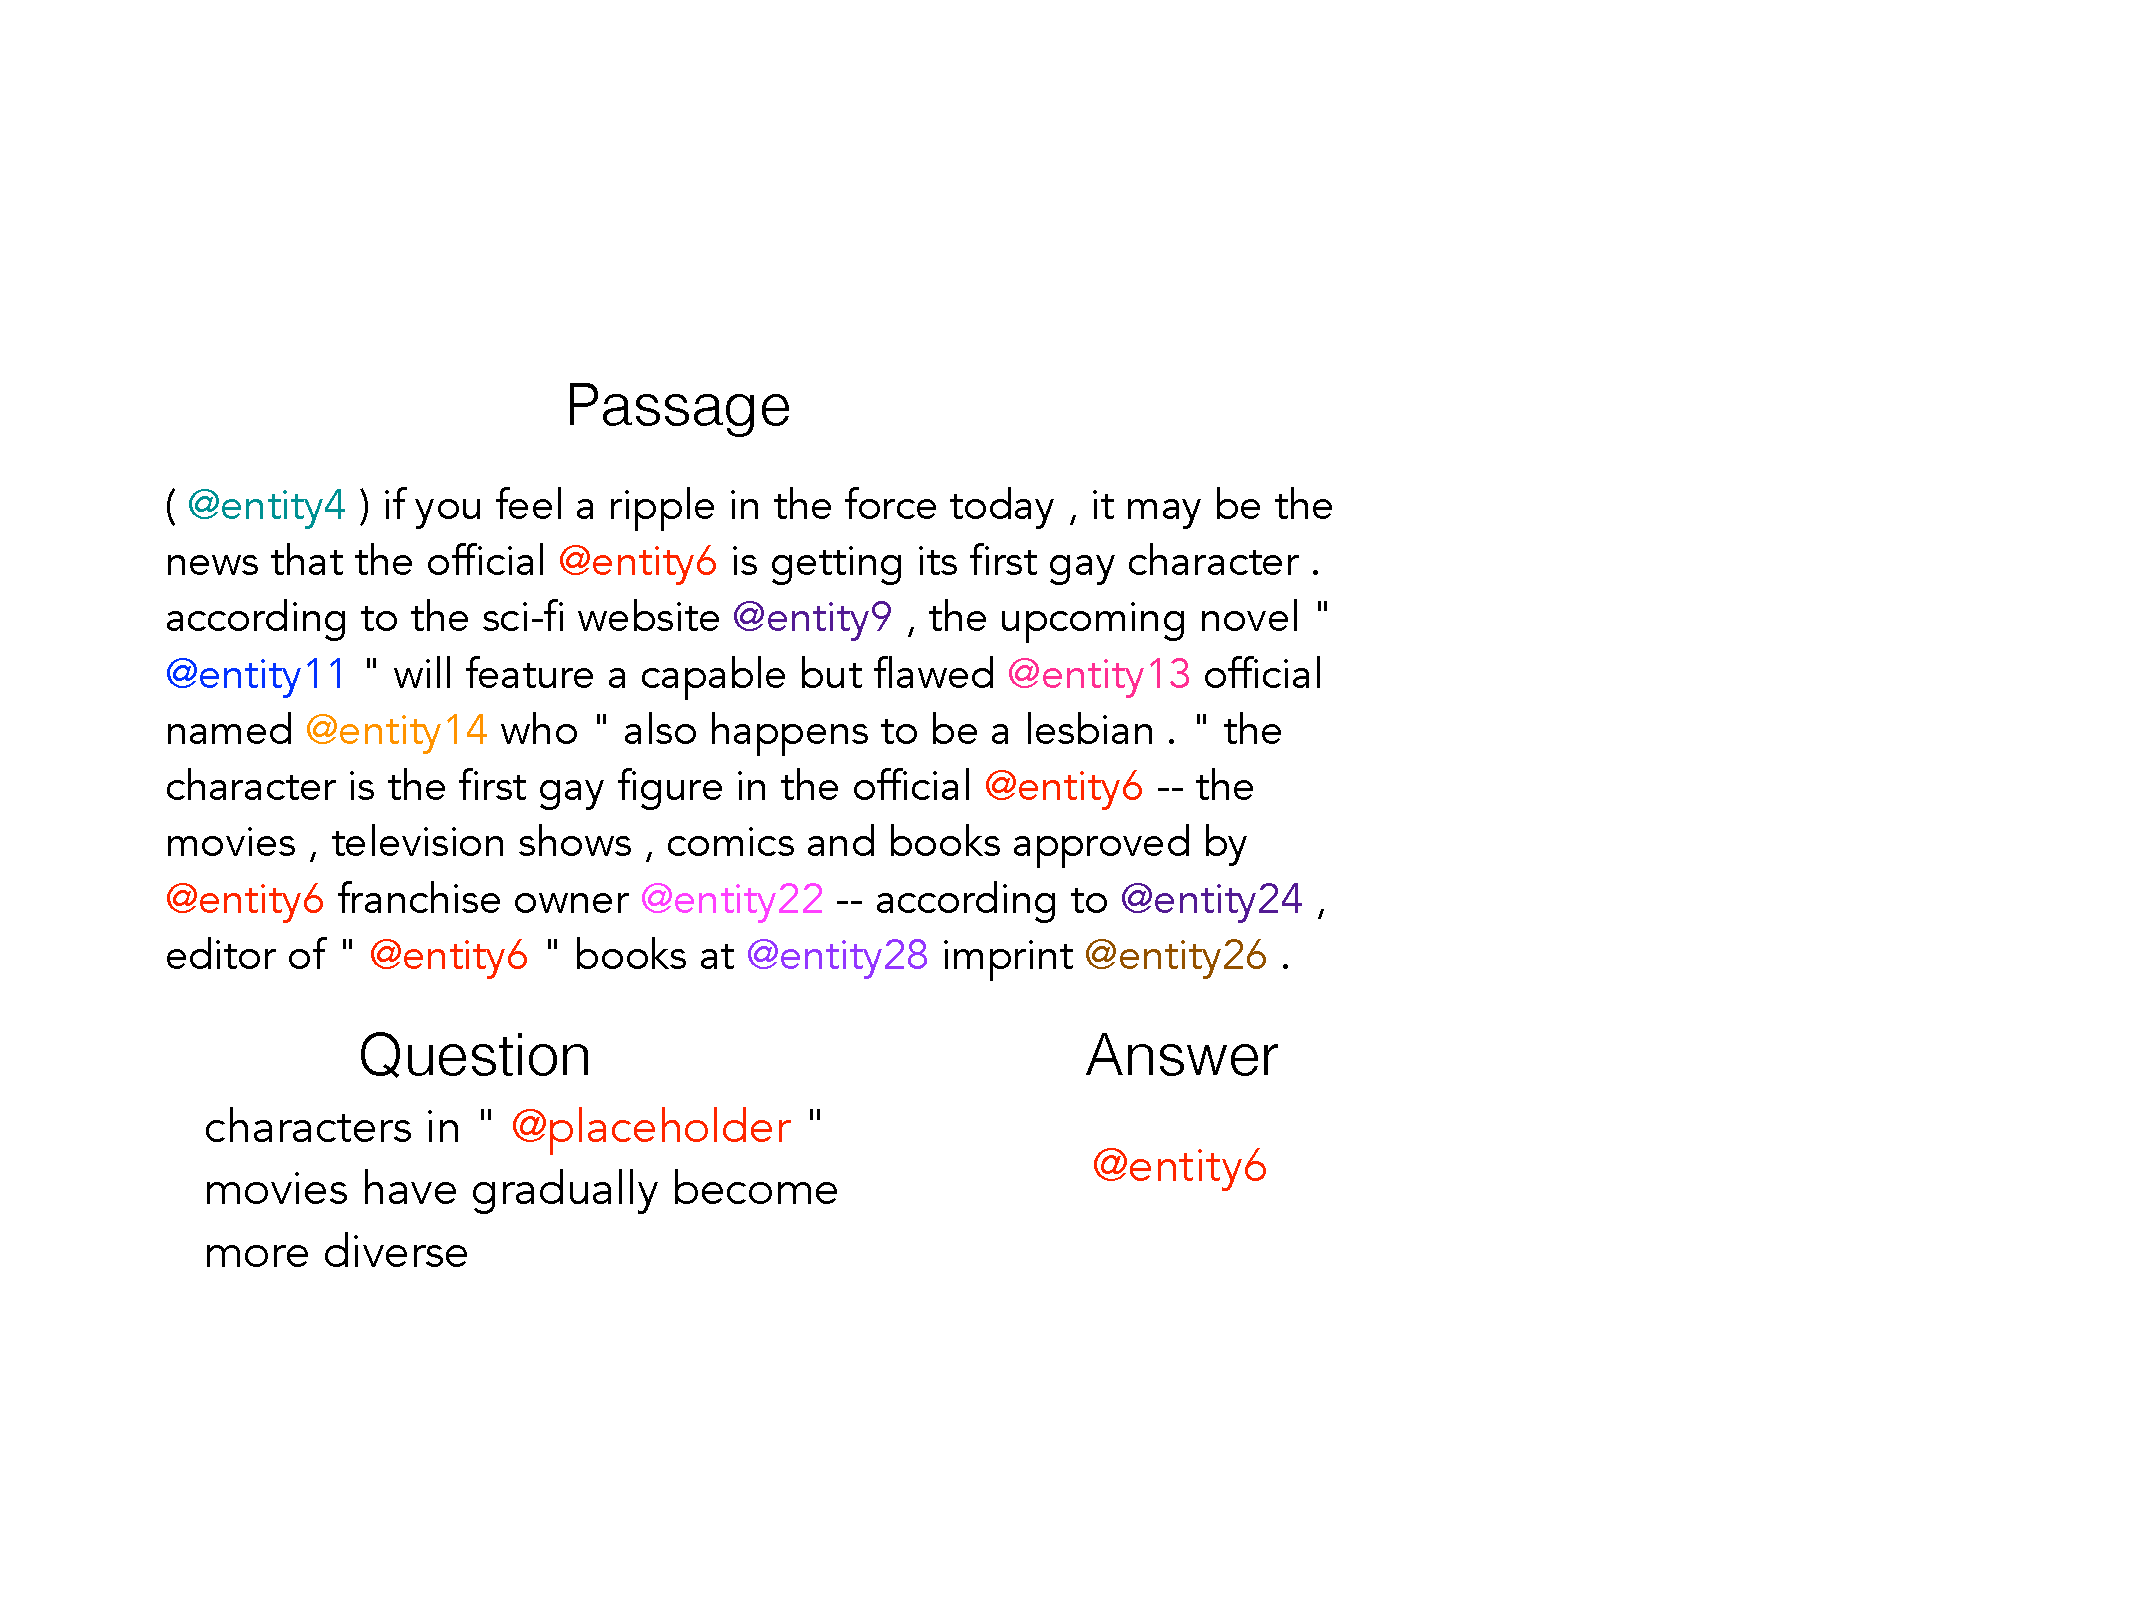
\includegraphics[scale=0.38]{figures/fig_example.pdf}
\vspace{-2em}
\caption{An example item from dataset \ti{CNN}.}
\label{fig:example}
\end{figure}

This is a clever way of creating supervised data cheaply and holds promise for making progress on training RC models; however, it is unclear what level of reading comprehension is actually needed to solve this somewhat artificial task and, indeed, what statistical models that do reasonably well on this task have actually learned.

In this paper, our aim is to provide an in-depth and thoughtful analysis of this dataset and what level of natural language understanding is needed to do well on it. We demonstrate that simple, carefully designed systems can obtain high, state-of-the-art accuracies of  {\finalcnn} and {\finaldm} on \ti{CNN} and \ti{Daily Mail} respectively. We do a careful hand-analysis of a small subset of the problems to provide data on their difficulty and what kinds of language understanding are needed to be successful and we try to diagnose what is learned by the systems that we have built.  We conclude that: (i)~this dataset is easier than previously realized, (ii)~straightforward, conventional NLP systems can do much better on it than previously suggested, (iii)~the distributed representations of deep learning systems are very effective at recognizing paraphrases, (iv)~partly because of the nature of the questions, current systems much more have the nature of single-sentence relation extraction systems than larger-discourse-context text understanding systems, (v) the systems that we present here are close to the ceiling of performance for single-sentence and unambiguous cases of this dataset, and (vi)~the prospects for getting the final 20\% of questions correct appear poor, since most of them involve issues in the data preparation which undermine the chances of answering the question (coreference errors or anonymization of entities making understanding too difficult).

